\documentclass[letterpaper,10 pt,conference,onecolumn]{IEEEtran}

% The following packages can be found on http:\\www.ctan.org
\usepackage{graphicx} % for pdf, bitmapped graphics files
\usepackage{epsfig} % for postscript graphics files
\usepackage{mathptmx} % assumes new font selection scheme installed
\usepackage{times} % assumes new font selection scheme installed
%\usepackage{amsmath} % assumes amsmath package installed
%\usepackage{amssymb}  % assumes amsmath package installed

%%%%%%%%%%%%%%%%%%%%%%%%%%%%%%%
% added packages 
%\usepackage {hyperref}
\usepackage {subfig}
\usepackage {subfloat}
\usepackage {xspace}
%% Math and symbol packages
\usepackage{amssymb}
\usepackage{amsmath}
%%% for kmap tables:
%\usepackage{hhline}
\usepackage{multicol}
%%% for \dashline
%\usepackage{epic}
\usepackage {enumerate}
\usepackage{scalefnt}
\usepackage{hyperref}
%%%%%%%%%%%%%%%%%%%%%%%%%%%%%%%%

\hypersetup{
	colorlinks, urlcolor=darkblue
}

% for cool graphics
\usepackage{pgf,tikz}
\usetikzlibrary{arrows,shapes.symbols,shapes.callouts,snakes,shapes.geometric}

\definecolor{darkblue}{cmyk}{1.0,0.7,0.0,0.2}
\definecolor{lightcyan}{cmyk}{0.5,0.0,0.0,0.0}
\definecolor{lightyellow}{cmyk}{0.0,0.0,0.5,0.0}
\definecolor{darkred}{rgb}{0.5,0.0,0.0}
\definecolor{lightblue}{rgb}{0.5,  0.5,  1.0}
\definecolor{lightblue}{rgb}{0.5,  0.5,  1.0}
\definecolor{darkgreen}{rgb}{0.0,  0.5,  0.0}
\definecolor{lightgreen}{rgb}{0.5, 1.0, 0.5}
\definecolor{deepred}{rgb}{0.8,0.00,0.00}


% Enter particular words to define specific hyphenation allowed
\hyphenation{}

\graphicspath{ {images/} }

% Process this with:
% pdflatex latex-template.tex
% bibtex latex-template.bib
% pdflatex latex-template.tex
% pdflatex latex-template.tex
\begin{document}

	\title{
		Parking Lot Guidance System Using Wireless Senor Modules and Cloud Processing
	}

	\author{
		\IEEEauthorblockN{
			Ben Figlin\IEEEauthorrefmark{1},
			Brennan Myers\IEEEauthorrefmark{2} and  
			Caelan Dailey\IEEEauthorrefmark{3}
		}
		\IEEEauthorblockA{
			Dept. of Electrical and Computer Engineering,
			University of Utah\\
			Email: \IEEEauthorrefmark{1}benfiglin@gmail.com,
			\IEEEauthorrefmark{2}brennan.myers@gmail.com,
			\IEEEauthorrefmark{3}caelandailey@gmail.com\\
			Website: \url{http://eng.utah.edu/~brennanm/website.html}
		}
	}

	\maketitle
	
	%%%%%%%%%%%%%%%%%%%%%%%%%%%%%%%%%%%%%%%%%%%%%%%%%%%%%%%%%%%%%%%%%%%%%%%%%%%%%%%%
	
	\begin{abstract}
	TODO!!
	\end{abstract}

	%%%%%%%%%%%%%%%%%%%%%%%%%%%%%%%%%%%%%%%%%%%%%%%%%%%%%%%%%%%%%%%%%%%%%%%%%%%%%%%%
	
	\section{Introduction}
		Driving a car to work or school is convenient when public transportation is either non-existent or consumes significantly more time. As more people use their cars, parking becomes a real issue and finding an available parking space can turn into a nightmare. We propose a solution to a significant portion of the problem by eliminating some of the unknowns and providing real-time insight into parking lot conditions, which will save both time and frustration. The solution will include a service through which users will be able to make instant decisions on when and where to park.
		
		Tracking available parking stalls will be achieved by developing and deploying a system capable of determining the percentage of available space through a method of counting the flow of vehicles into and out of a parking lot. By using custom hardware and commonly used sensors, data will be captured and pushed to our cloud service. Vehicle traffic will be counted by remote modules at each entrance. Each remote module will have a battery and a solar panel to simplify installation where no power is available. The data will then be transmitted wirelessly (through low-frequency RF) to a base station which will collect the information and push it to a cloud service over the internet. Advanced analysis within our cloud will take into account previous parking lot conditions and will predict how full a lot will be at any given time. A mobile application connected to the cloud will then use this data to provide a graphical representation of the parking lot. The resulting system will provide peace of mind to drivers by enabling easy access to real-time conditions, historical trends and useful predictions through a simple web interface or a mobile app.
		
		Our team possesses a variety of skills that can be applied directly to this project. We are passionate about electrical and computer design, which has become second nature to us. This project will become a reality by applying our expertise in embedded systems, networking, and mobile app development. Using these skills, together with dedication and hard work, we will provide a smart solution that will simplify parking for all.

	\section{Background}
		Multiple approaches exist to the challenge of parking lot metering. Some solutions propose metering individual stalls, while others suggest counting differential traffic to and from a parking lot. While the former presents a very accurate solution, it involves high complexity and cost due to the need of sensor electronics at each individual stall and a way to communicate between them all. The latter is easy to integrate and requires very few sensors and supporting hardware, but is slightly less accurate and may require recalibration maintenance from time to time.
		
		Our project will be focusing on the differential approach for reasons of cost effectiveness and simplicity, making it a practical solution for mass implementation. With that approach, different sensing techniques exist, each with its advantages and disadvantages. We examined various existing products that are similar to our proposed solution and arranged them into three categories by their sensing technology. Some of those products are mentioned below:
		
		\subsection{Inductive Loop Solutions}
			\textbf{T2Systems AutoCount} - The system uses in-ground inductive loops at each entrance and exit for counting inbound and outbound traffic. The sensor units are self powered using solar panels. One disadvantage is the difficult installation which requires placing inductive loop wires into the road. Another disadvantage is the low accuracy of inductive loops which requires syncing the system very often \cite{autocount}.
	
		\subsection{Optical and Ultrasonic Solutions}
			\textbf{Signal-Tech RedStorm} - The product incorporates two IR overhead sensors for each lane which detect overlap and are able to detect direction of movement while also ignoring smaller objects like pedestrians. Some of the disadvantages include: (1) Sensors can be mounted in an overhead configuration only and therefore are less suitable for places where no ceiling exists above the lanes, and (2) Modules must be wired to communication and power, which complicates installation where power is not available and increases the cost due to the needed extra infrastructure \cite{redstorm}.
		
		\subsection{Video Processing Solutions}
			\textbf{Mirame TrueView Parking} - This system uses a ceiling mounted camera to detect traffic on both the inbound and the outbound lane of a parking lot entrance/exit. Each camera does the signal processing and the counting on-board and communicates directly through the internet. This solution is somewhat more expensive due more complex electronics and can be only mounted in an overhead configuration \cite{trueview}.
	
	\section{Proposed Work}
		\subsection{System Overview}
			The proposed project will be based on a differential counting of the vehicles going into and out of a parking lot. Counting will be done by wireless sensor modules located at each entrance and exit point. Each module will consist of a sensor (or a pair of sensors), an RF transceiver, a small microprocessor board, a battery, and a solar panel. All modules will be communicating with a base unit which will be receiving raw data over RF and will be sending that data to the Internet-based backend server. Data will be processed and stored in the server, and will be accessed by user friendly apps or a web interface. Figure \ref{fig:overview} shows, at a high level, the different components of the system and how they interconnect.
			
			\begin{figure}[h]
				\centering
				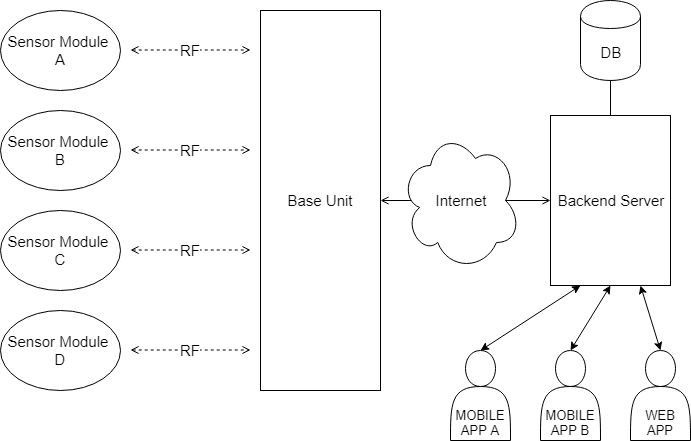
\includegraphics[width=0.65\columnwidth]{overview}
				\caption{A high level block diagram of the proposed system}
				\label{fig:overview}
			\end{figure}
		
		\subsection{Vehicle Sensing}
		
		\subsection{Communication}
		
		\subsection{Power}
		
		\subsection{Backend Server}
		
		\subsection{User Interface}
		
	\section{Schedule}
		
		
	\section{Resources}
		
		
	\section{Summary}
 		
		
	%%%%%%%%%%%%%%%%%%%%%%%%%%%%%%%%%%%%%%%%%%%%%%%%%%%%%%%%%%%%%%%%%%%%%%%%%%%%%%%%
	%\begin{multicols*}{2}
	\bibliographystyle{IEEEtran}
	\bibliography{references}
	%\end{multicols*}
	
\end{document}